%%%%%%%%%%%%%%%%%%%%%%%%%%%%%%%%%%%%%%%%%%%%%%%%%%%%%%%%%%%%%%%%%%%%%%%%%%%%%%%%
%2345678901234567890123456789012345678901234567890123456789012345678901234567890
%        1         2         3         4         5         6         7         8

\documentclass[letterpaper, 10 pt, conference]{ieeeconf}  % Comment this line out if you need a4paper

%\documentclass[a4paper, 10pt, conference]{ieeeconf}      % Use this line for a4 paper

\IEEEoverridecommandlockouts                              % This command is only needed if 
                                                          % you want to use the \thanks command

\overrideIEEEmargins                                      % Needed to meet printer requirements.

% See the \addtolength command later in the file to balance the column lengths
% on the last page of the document

% The following packages can be found on http:\\www.ctan.org
%\usepackage{graphics} % for pdf, bitmapped graphics files
%\usepackage{epsfig} % for postscript graphics files
%\usepackage{mathptmx} % assumes new font selection scheme installed
%\usepackage{times} % assumes new font selection scheme installed
\usepackage{amsmath} % assumes amsmath package installed
%\usepackage{amssymb}  % assumes amsmath package installed
\usepackage{url}
\usepackage{graphicx}
\usepackage{color}

\usepackage{soul}

\graphicspath{{./images/}}

%\pdfminorversion=4

\title{\LARGE \bf
Improving Condition- and Environment-Invariant Place Recognition with Semantic Place Categorization
}

\author{Sourav Garg$^{1}$, Adam Jacobson$^{1}$, Swagat Kumar$^{2}$ and Michael Milford$^{1}$% <-this % stops a space
\thanks{$^{1}$The authors are with Australian Centre for Robotic Vision,
        Queensland University of Technology,
        2 George St, Brisbane, Australia}%
\thanks{$^{2}$The author is with Innovation Labs, Tata Consultancy Services,
        New Delhi, India}%
}


\begin{document}



\maketitle
\thispagestyle{empty}
\pagestyle{empty}

%%%%%%%%%%%%%%%%%%%%%%%%%%%%%%%%%%%%%%%%%%%%%%%%%%%%%%%%%%%%%%%%%%%%%%%%%%%%%%%%

\begin{abstract}
The problem of place recognition actually comprises two distinct subproblems; ``traditional'' place recognition which is recognizing a specific location in the world, and place ``categorization'', which involves recognizing the type of place. Both components of place recognition are competencies for robotic navigation systems and hence have each in isolation received significant attention in the robotics and computer vision community. In this paper, we leverage the powerful complementary nature of the place recognition and place categorization processes to create a new state-of-the-art traditional place recognition system that uses place context to inform place recognition. We show that semantic place categorization creates a more informative natural segmenting of physical space than the blindly applied fixed segmentation used in algorithms such as SeqSLAM, which enables significantly better place recognition performance. In particular, where existing condition-invariant algorithms enable robustness to globally consistent change (such as day to night cycles), this new semantically informed approach adds robustness to significant changes within the environment, such as transitioning from indoor to outdoor environments. We perform a number of experiments using benchmark and new datasets and show that semantically-informed place recognition outperforms the previous state-of-the-art systems. Like it does for object recognition \cite{sunderhauf2016place}, we believe that  semantics can play a key role in boosting conventional place recognition and navigation performance for robotic systems.
\end{abstract}
%%%%%%%%%%%%%%%%%%%%%%%%%%%%%%%%%%%%%%%%%%%%%%%%%%%%%%%%%%%%%%%%%%%%%%%%%%%%%%%%

%%%%%%%%%%%%%%%%%%%%%%%%%%%%%%%%%%%%%%%%%%%%%%%%%%%%%%%%%%%%%%%%%%%%%%%%%%%%%%%%
\section{INTRODUCTION}


The problem of traditional place recognition typically focuses on recognizing specific locations in the world stored within a database of ``places''. This form of place recognition is very powerful, enabling localization on very large scales~\cite{Cummins2009} and during difficult day and night traverses of an environment~\cite{Milford2012}. The problem of place categorization is similar to the place recognition problem, where environments are evaluated to determine the type of place from a database of place types. 

We see the problem of place categorization as an extension to the place recognition problem, where it is possible to use similar frameworks to solve both problems. We highlight the main differences in application between the two approaches, noting that within place recognition frameworks, the goal is to identify and utilize differences between locations within the dataset to enable unique localization. Place categorization algorithms highlight the similarity between intra-class samples to create a comprehensive representation of a particular place type and are expected to be able to generalize class labels to classify and extend to unseen environments. The place categorization framework typically utilizes less ``labels'' than place recognition and more training examples of what represents a particular place category whereas place recognition has a ``label'' within a database representing every location in the environment. 

\begin{figure}
	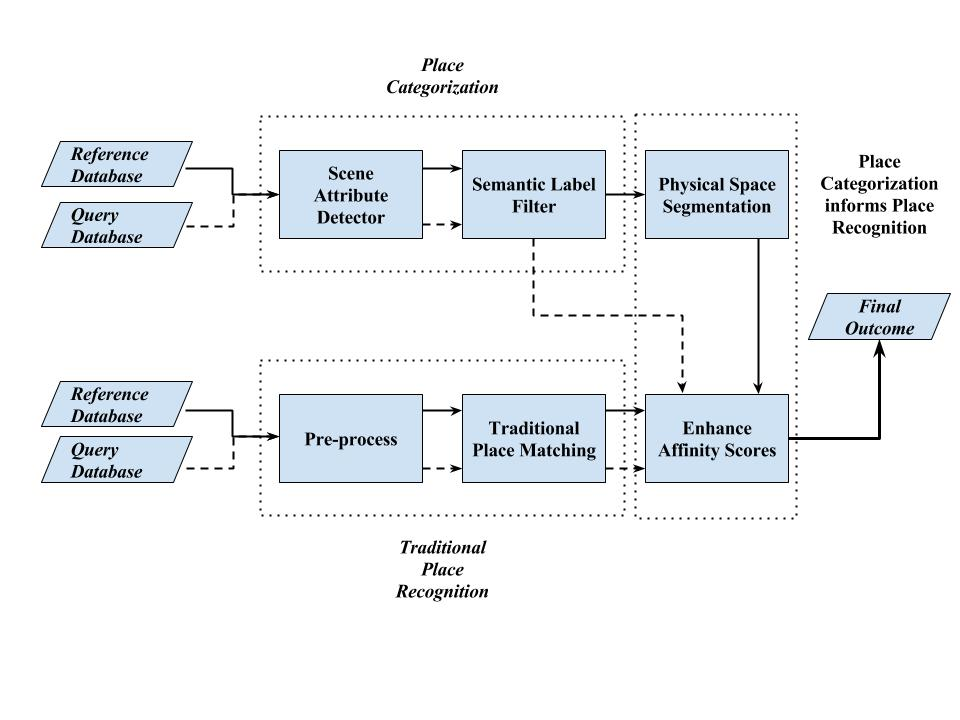
\includegraphics[clip, trim=1cm 4cm 0cm 2cm,scale=0.26]{flowchart}
	\caption{A block diagram showing the flow of semantic information from the place categorization module to the place recognition module for better performance.}
	\label{fig:flowchart}
\end{figure}


In this work, we combine the two frameworks of place recognition and place categorization to improve place recognition localization performance. Our primary contribution is the development of a novel framework to incorporate semantic labels and place categorization results to inform and improve place recognition place estimates (as seen in Fig.~\ref{fig:flowchart}).  
Once a place is categorized, we leverage the SeqSLAM framework to perform place recognition, implementing a novel dynamic weighting scheme, biasing place matches with similar place characteristics and place categorization results. 

We evaluate our proposed approach within the two real world datasets, the Campus Dataset and the CTA-Rail Dataset. The Campus Dataset utilizes a single camera traversing indoor and outdoor campus environments and the CTA-Rail Dataset consists of a single camera mounted on a train traversing scenes with subway station platforms, subway tunnels and railroad tracks. The proposed approach, incorporating place categorization information,  outperforms a standalone state-of-the-art place recognition system in both the environments.  

The paper proceeds as follows. In Section 2, we review literature with a focus on place recognition and place categorization. Section 3 presents our approach describing the implementation of our CNN place categorization framework, outlines our place recognition framework and the proposed technique for combining the two frameworks to produce superior place recognition results. We present the experimental setup in Section 4, and results of multiple levels of evaluation in Section 5. Section 6 discusses the significance of the research and areas of future work.

\section{Related Work}
In this section, we review current research in the areas of place categorization and place recognition. We specifically focus on place recognition, semantic mapping and place categorization frameworks. 

\subsection{Place Recognition}
Visual place recognition leverages a visual map of the environment and compares visual information, typically from a camera sensor, with the map data to determine the current location of the camera within the map. There are many techniques which have been proposed to solve this problem of determining where an image has been taken within an environment. Typically, these approaches leverage single frame matching to determine the location of the camera in the environment. The key goal of place recognition frameworks is to separate places in the environment and highlight the unique attributes or features which uniquely describe individual locations in the environment~\cite{Cummins2009,nister2006scalable}. 

There have been many attempts to improve performance of place recognition systems. This has included the inclusion of temporal information, fusing multiple sensory modalities and implementing unique preprocessing steps to improve localization capabilities like shadow removal techniques. 

Temporal information has been incorporated into the place recognition framework with the introduction of the SeqSLAM framework~\cite{Milford2012}, integrating place hypotheses over small distances to accrue evidence and improve place recognition performance.

Multi-sensor fusion has been investigated in a number of works~\cite{tapus2006cognitive,Milford2013a}, attempting to introduce unique sensory modalities which have different failure modes to produce robust place estimates. 

Furthermore, the introduction of unique sensor preprocessing techniques to improve sensor data for place recognition has also been explored. Frameworks utilizing techniques for shadow removal~\cite{corke2013dealing} or the introduction of illumination invariant color spaces~\cite{mcmanus2014shady} to remove temporal or environmental changes from images to improve localization. 

The work presented in place categorization attempts to develop the generic capability to identify types of places in the world, potentially enabling improvements in place recognition capabilities. 

%What is evident from the work presented in [Smart Paper] is that additional information 

\subsection{Place Categorization}

Place categorization systems are an extension of the place recognition problem and attempt to attach semantic meaning to particular places in an environment; attempting to utilize labels from a training set like indoor, outdoors, kitchen, office and bedroom to categorize the location within which an image was taken. These frameworks are powerful as they facilitate generalization of room labels to different environments, for example identifying a bedroom within an unexplored house, potentially enabling robotic platforms to perform generic tasks in unknown environments by recognizing the type of place~\cite{wu2009visual}. 

There have been a number of works which attempt to imbue traditional SLAM architectures with the ability to semantically label locations in an environment\cite{sunderhauf2016place, ranganathan2011visual}. These types of frameworks utilize the place categorization labels to provide information about a space, for example a location is mostly likely a kitchen, but these labels are not utilized in the process of generating the map or performing place recognition or localization. 

In a recent work \cite{mohan2015environment}, authors develop a method to generate different categories of environments from a large available reference database for place recognition in order to reduce the search space for matching places. They basically segment the overall physical space into categories of similar environments within the place recognition system and do not use any semantic place categorization.

Place categorization systems have been leveraged in previous work to improve object detection and classification, enabling reduction of the object search space and improvement in object recognition performance~\cite{torralba2003context}. 

However, there has been no prior work utilizing place categorization information to improve place recognition place estimates. 

%\hl{Emphasize the generalization capability of categorization over place rec  - Maybe echo earlier. }

%\hl{I dont have any background in this. If you have a particular message you want to get across here, let me know and I can try to write something. }


\section{Proposed Method}
The proposed approach has three main components: place categorization, physical space segmentation and place recognition as depicted in Fig. \ref{fig:flowchart}, with semantic information flowing from the former to the latter to generate the final place match estimate. Our core contribution is the development of a technique to utilize place categorization information to improve place recognition performance. In order to achieve this, we use the semantic labels to divide the physical space into different regions based on its appearance, that is, scene attributes. These segmented regions along with semantic labels are then incorporated in the place recognition module for biasing place matches with similar place characteristics and place semantics. We use CNN model VGG16-places365 \cite{cnnPlaces365Github} pre-trained on the Places365 database \cite{zhou2014learning} for labeling reference and query database frames with most probable scene attributes \cite{Patterson2012SunAttributes}. We use SeqSLAM \cite{Milford2012} for showing improved place recognition using semantic information by appropriately enhancing the image matching scores.

\subsection{Place Categorization}

\newcommand{\scaleVal}{0.27}
\begin{figure*}
	\centering
	\begin{tabular}{ccc}
		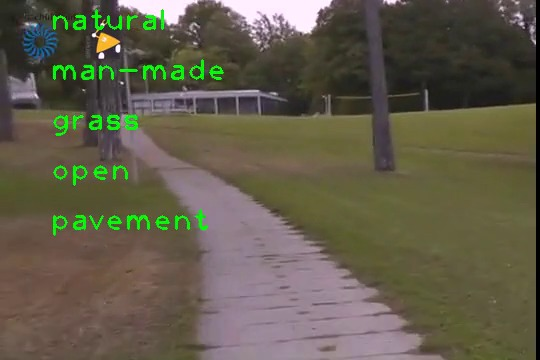
\includegraphics[scale=\scaleVal]{1-outdoor} &
		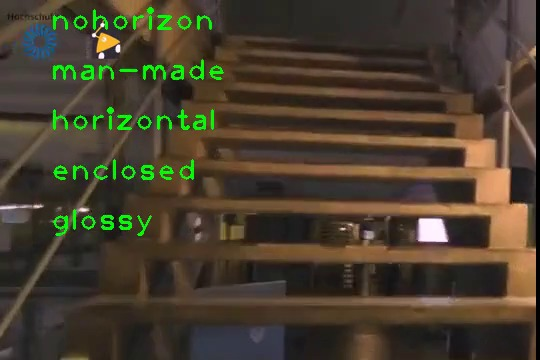
\includegraphics[scale=\scaleVal]{2-stairs} &
		%  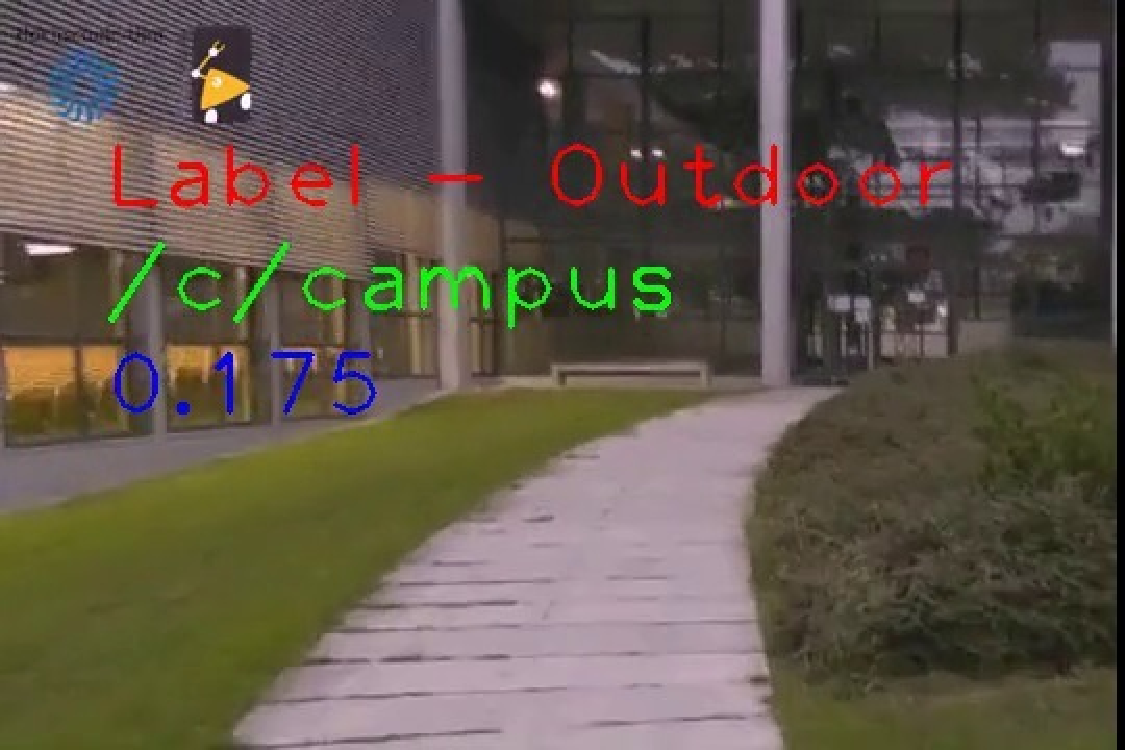
\includegraphics[scale=\scaleVal]{3-campus} &
		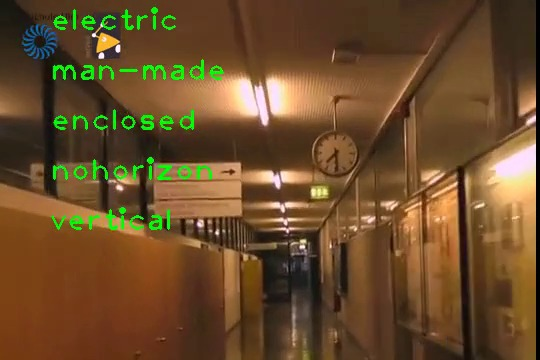
\includegraphics[scale=\scaleVal]{3-indoor} \\
		%  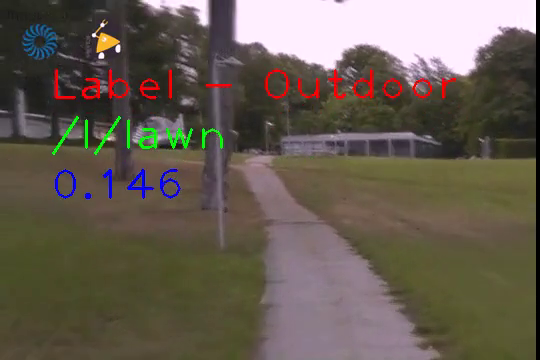
\includegraphics[scale=\scaleVal]{5-lawn} &
		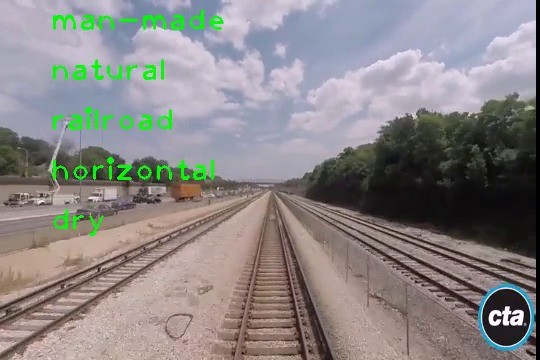
\includegraphics[scale=\scaleVal]{4-railroad} &
		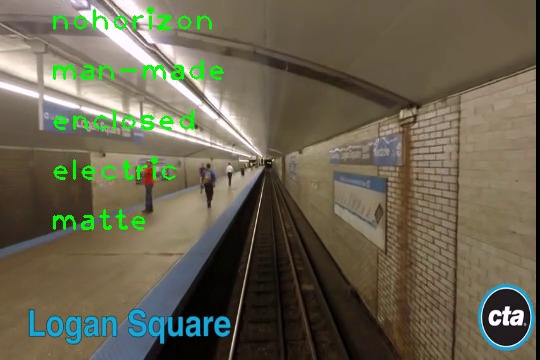
\includegraphics[scale=\scaleVal]{5-subway} &
		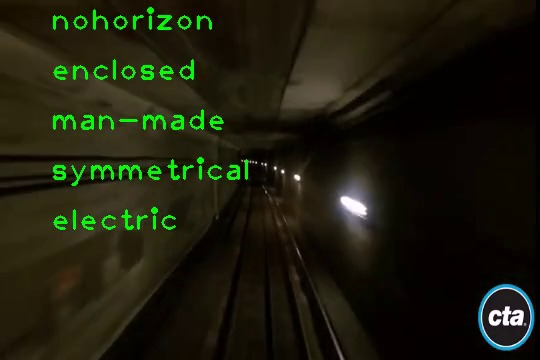
\includegraphics[scale=\scaleVal]{6-tunnel} \\
	\end{tabular}
	\caption{Images from reference database with top-5 most probable semantic labels out of 102 scene attributes for Campus Dataset (top) and CTA Rail Dataset (bottom).}
	\label{fig:labelledImages}
\end{figure*}

The pre-trained CNN model classifies an image with probabilities associated with each of the 365 place categories. It is also made to predict the most probable scene attributes (out of 102 attributes trained on the SUN database \cite{Patterson2012SunAttributes}) using one of its fully-connected layers. We use the top-5 most probable attribute predictions for post-processing the image labels to semantically segment datasets. The predicted scene attributes for some of the images from datasets used in this paper are shown in Fig. \ref{fig:labelledImages}. The classification is performed on the entire reference and query database. The reference database labels are used for temporally dividing the image sequence into different chunks based on its scene attributes. The query database labels are used later during place recognition for identifying the correct semantic segment of reference database and effectively matching the image sequence.

\subsection{Physical Space Segmentation}
The image labels for reference database obtained from the classifier usually do not exhibit local temporal consistency. In order to achieve an adequate physical space segmentation, we find temporal connected components in the database. Each image in the database is represented by a node $N_i$ defined as a set containing the top-5 predicted labels and the most probable prediction label $L_i$. A consecutive pair of nodes is considered to be connected if an edge $E_{i,i+1}$ exists between them as per Eq. \ref{eq:connectedComponent}.
\begin{equation}
 E_{i,i+1} = 
 \begin{cases}
  1, & \text{if } \left\vert{N_i \cap N_{i+1}}\right\vert \geq 3\\
  0, & \text{otherwise}
 \end{cases}
 \label{eq:connectedComponent}
\end{equation}

The edges between the nodes can be determined by a single pass over the entire image sequence. A new connected component $c_k = \{N_{c_k},N_{c_{k+1}}\}$ is obtained whenever an edge between consecutive nodes ceases to exist, where $N_{c_k}$ and $N_{c_{k+1}}$ are the nodes marking the beginning and end of the connected component. The most probable prediction label $L_i$ of each node in a connected component is used to find the most frequently occurring label $L'_i$ within that component. 
\begin{equation}
 L'_i = mode(\biguplus\limits_{i=N_{c_k}}^{N_{c_{k+1}}} L_i) \hspace{0.5cm} \forall k
  \label{eq:labelsModeCC}
\end{equation}
where $k$ iterates over connected components and $mode(X)$ for a set $X$ gives its statistical mode.

This label $L'_i$ is used for representing the connected component as well as each of its nodes. These newly obtained labels are further filtered to get rid of transient errors and merge some of the consecutive components. We use a sliding window of size $s$ that passes through the entire image sequence and replaces the label $L'_i$ by the mode of labels within the sliding window as given in Eq. \ref{eq:labelsMode}.
\begin{equation}
 \hat{L}_i = mode(\biguplus\limits_{i-s/2}^{i+s/2} L'_i)
 \label{eq:labelsMode}
\end{equation}

For sake of clarity, it can be noted that labels $L'_i$ are obtained by looking at the labels of individual nodes of a connected component and are then assigned to that component and its participating nodes, whereas, the labels $\hat{L}_i$ are obtained by looking at the individual nodes of the entire database and then assigned to that particular node itself where the sliding window is centered. The purpose of the former is intra-component label consistency while the latter is for inter-component label consistency.

The filtered image labels $\hat{L}_i$ are finally used to segment the database into $M$ chunks represented as $C_K = \{N_{C_K},N_{C_{K+1}}\}$, where $N_{C_K}$ and $N_{C_{K+1}}$ are the nodes that mark the beginning and end of the data chunk. The label corresponding to each chunk is the same as the label for all its nodes and is represented as $\hat{L}_{C_K}$. These chunks represent the variation in appearance of the environment while traversing the route. For example, a train running underground as opposed to over the ground will have different appearance of its environment. Similarly, a person walking indoor or outdoor of a campus will witness different surrounding environment as shown in Fig. \ref{fig:labelledImages}. Fig. \ref{fig:datasetLabels} shows the images and their semantic labels at the segmentation transition points for one of the datasets used in this paper.

\begin{figure}
 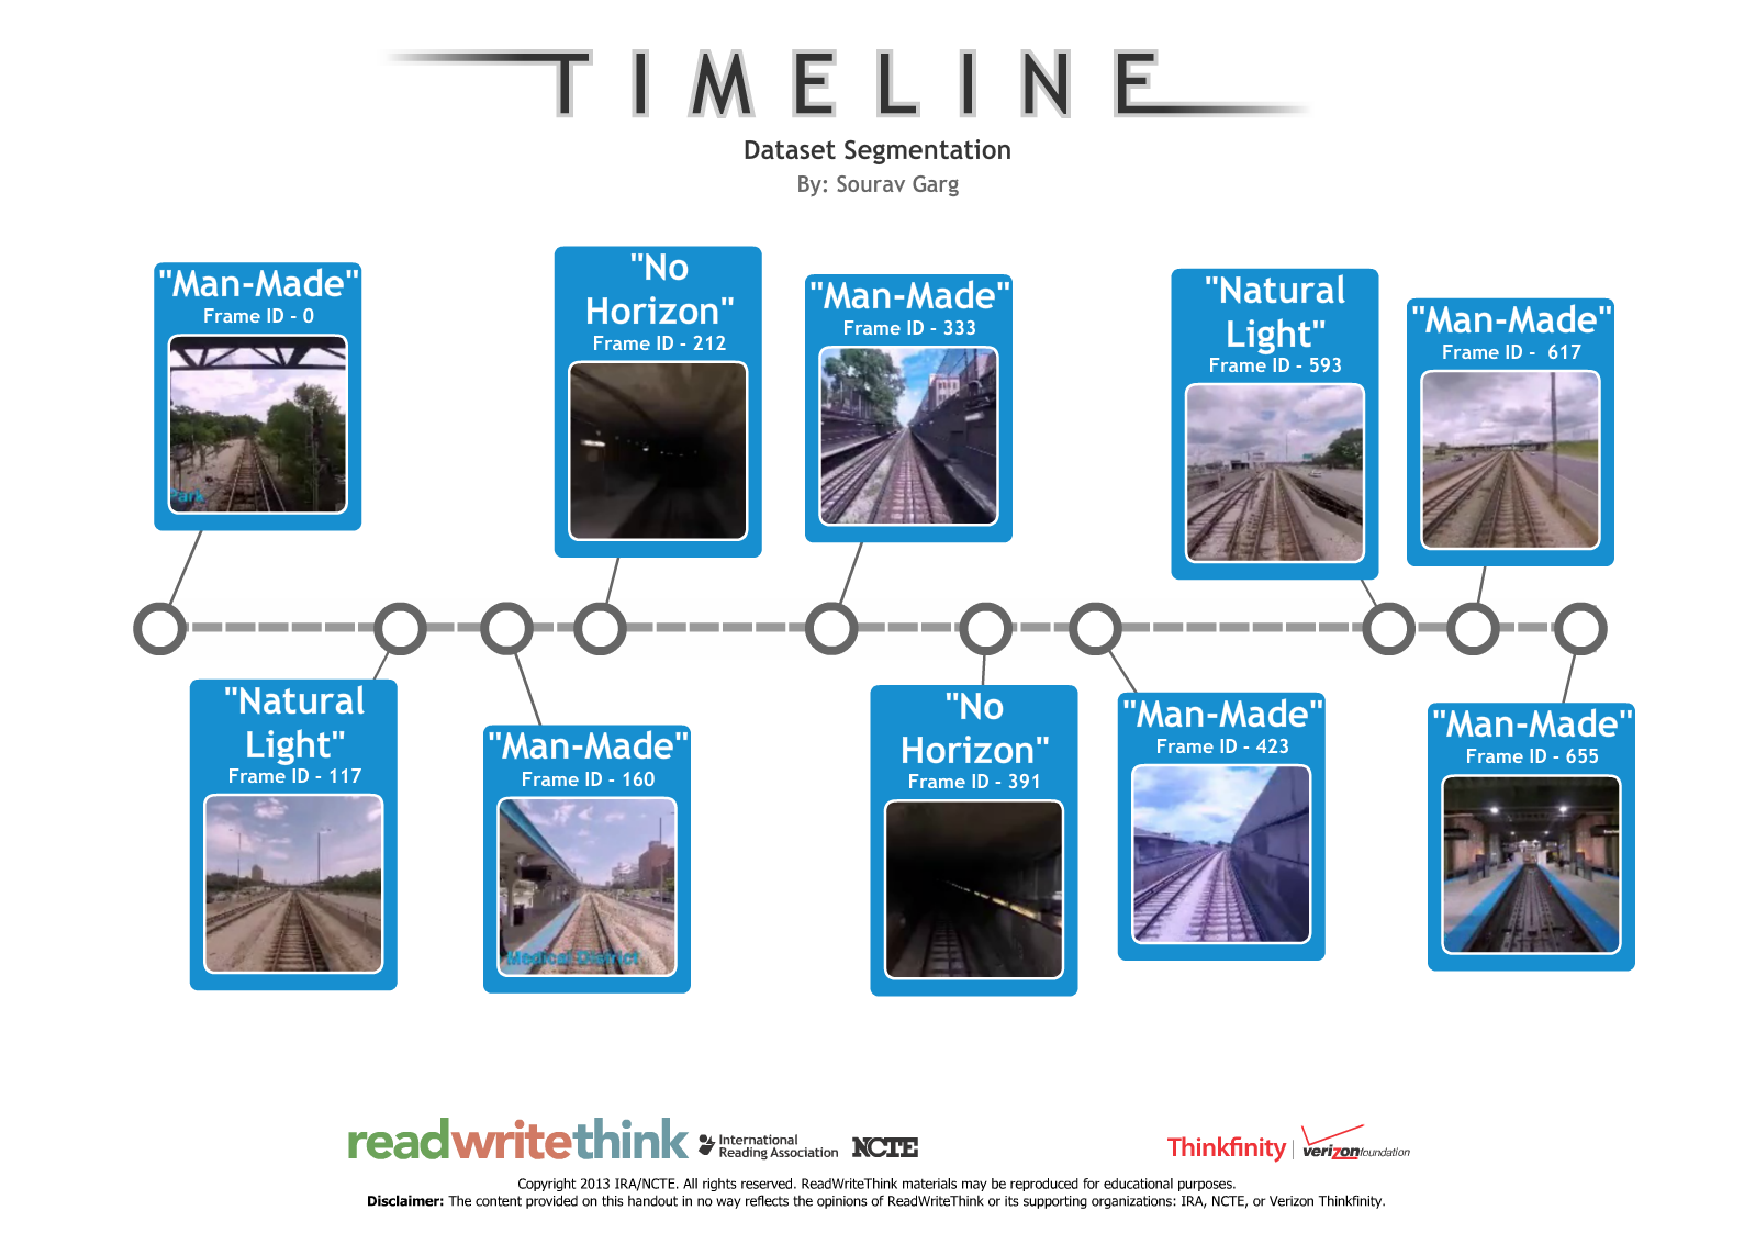
\includegraphics[clip, trim=2cm 4cm 2cm 4cm,scale=0.32]{cta-dataset-segmentation-1}
 \caption{The time-line of CTA-Rail dataset with semantically labeled images at the transition points of segmented reference database. (Time-line created using \cite{timelineRWT})}
 \label{fig:datasetLabels}
\end{figure}

\subsection{Place Recognition}
In general, a place recognition system comprises of a pre-processing stage, then a method to calculate affinity scores between database places and the query, and finally a decision module for generating the best matching pairs, as seen in Fig. \ref{fig:flowchart}.
\subsubsection{Sequence-based place matching}
In addition to the above mentioned place recognition pipeline, a sequence-based recognition method exploits the temporal information inherent in this problem. Therefore, searching for a matching sequence of places is a better approach than deciding a match based only on single matching template from reference imagery. SeqSLAM \cite{Milford2012} is a sequence-based place recognition method developed on similar principle. Moreover, it is known to work remarkably well in challenging environmental conditions and is able to recognize places despite seasonal, weather or time of day variations. The recent advanced methods \cite{milford2015sequence}, \cite{wang2015improved}, \cite{milford2015place} etc. inspired from SeqSLAM further improve the state-of-the-art for place recognition. In this paper, we use the vanilla approach to show the performance improvement of a place recognition system, under the influence of variations in the surrounding environment, with the help of semantic information associated with those places. The detailed methodology of SeqSLAM can be referred to in \cite{Milford2012}.

SeqSLAM performs place recognition using Sum of Absolute Difference (SAD) scores represented as $D$ between preprocessed reference and query images. The preprocessing step involves down-sampling of image to size $S_x$ and $S_y$ and patch normalizing it with a fixed square window of side length $P$.
\begin{equation}
 D_i = \frac{1}{S_xS_y} \sum\limits_{x=0}^{S_x}\sum\limits_{y=0}^{S_y}|p_{x,y}^j-p_{x,y}^i|
 \label{eq:SADscore}
\end{equation}
where $p_{x,y}^i$ and $p_{x,y}^j$ are the pixel intensities of patch normalized reference and query images.

The difference vector obtained for each query image undergoes neighborhood normalization within a sliding window of size $R$, also termed as neighborhood normalization zone width. The neighborhood normalized difference for a given query image, $\hat{D_i}^R$ is calculated using the local mean difference $\bar{D_i}^R$ and local standard deviation $\sigma_i^R$.
\begin{equation}
 \hat{D_i}^R = \frac{D_i-\bar{D_i}^R}{\sigma_i^R}
 \label{eq:normScore}
\end{equation}

The neighborhood normalized SAD matrix is then searched for local image sequence trajectories of length $d_s$, within a limited range of velocities, originating from each of the reference image. The sequence trajectory with the best score is then selected using a trajectory uniqueness threshold $\mu$.

\subsubsection{Implicit dataset segmentation}
The neighborhood normalization of place matching scores within the window $R$, as calculated in Eq. \ref{eq:SADscore} and \ref{eq:normScore}, reflects the emphasis on matching a local physical region of the environment. The parameter $R$ represents the span of environment, where the matching scores are locally enhanced. Our aim is to pre-define these physical regions of the environment for effectively matching the places that share similar semantic labels. The subsequent section shows how this can be achieved using the place recognition method chosen above.

\subsubsection{Semantically-informed place matching}
The segmentation of the dataset as described in earlier sections using the consistency of semantic labels, is a way of separating the physical space into regions with similar environmental conditions. As shown in Fig. \ref{fig:flowchart}, in general, a place recognition system can use the semantic information from the place categorization module to enhance its affinity scores for matching places. We show the effect of this by implementing it for the place recognition method - SeqSLAM as described below.

The first step towards exploiting the segmented regions of the reference database and semantic labeling is to find the region candidates that have the same label as the query image. This is achieved by simply matching the labels of the segmented regions, $\hat{L}_{C_K}$ and the query image label $\hat{L}_j$. For a given query image $N_j$, these region candidates are used to define the neighborhood ranges in the reference database for normalization purpose:
\begin{equation}
\begin{split}
 R'_i = \{\{N_{C_K},N_{C_{K+1}}\}\mid\hat{L}_{C_K}=\hat{L}_j \text{ and } \\
 i\in\{N_{C_K},N_{C_{K+1}}\} \} \hspace{0.2cm}\forall K
\end{split}
\end{equation}
where $i$ iterates over all the reference images, $K$ iterates over all the segmented regions, and $R'_i$ is the set of pairs of nodes that define the range for neighborhood normalization. If $R'_i$ happens to be a null set, then the vanilla method is used, otherwise:

\begin{equation}
 \hat{D_i}^{R'_i} = \frac{D_i-\bar{D_i}^{R'_i}}{\sigma_i^{R'_i}} \hspace{0.2cm}
 \label{eq:normScoreNew}
\end{equation}

Fig. \ref{fig:SADmatRdisplay} shows the method described in this section for choosing $R$. The incorporation of segmented regions based neighborhood normalization as shown, makes the appropriate use of semantic information by handling the different physical environments separately.

\begin{figure}
 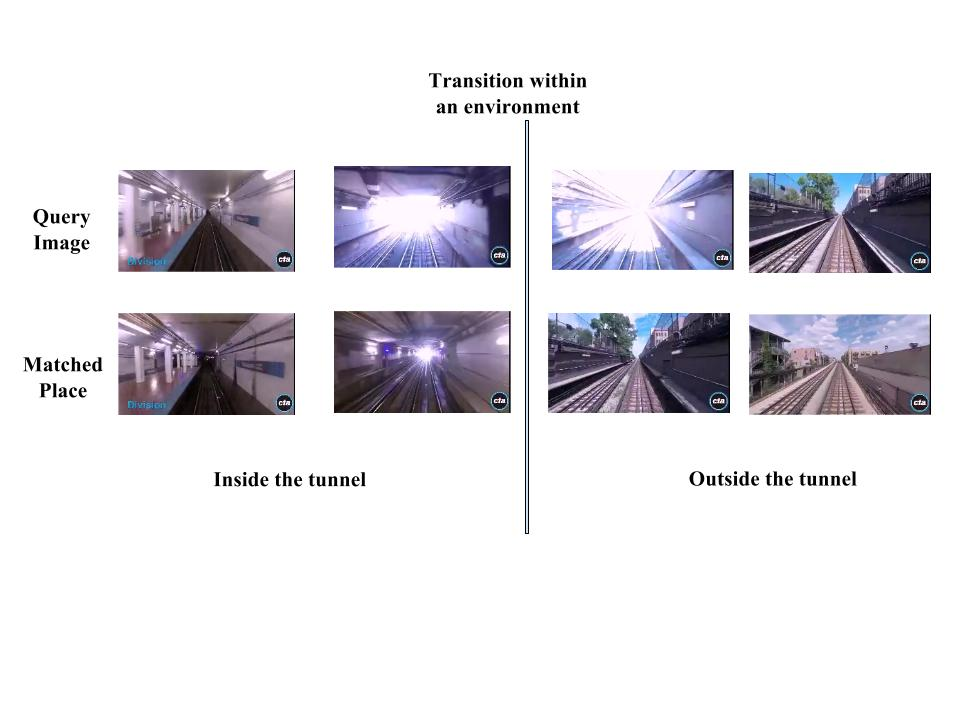
\includegraphics[clip, trim=3cm 7cm 0cm 2cm,scale=0.28]{PlaceMatchesAtTransition}
 \caption{Matched places at the point of transition within an environment for CTA-Rail dataset (top) and Campus Indoor-Outdoor dataset (bottom).}
 \label{fig:placeMatches}
\end{figure}


\begin{figure}
 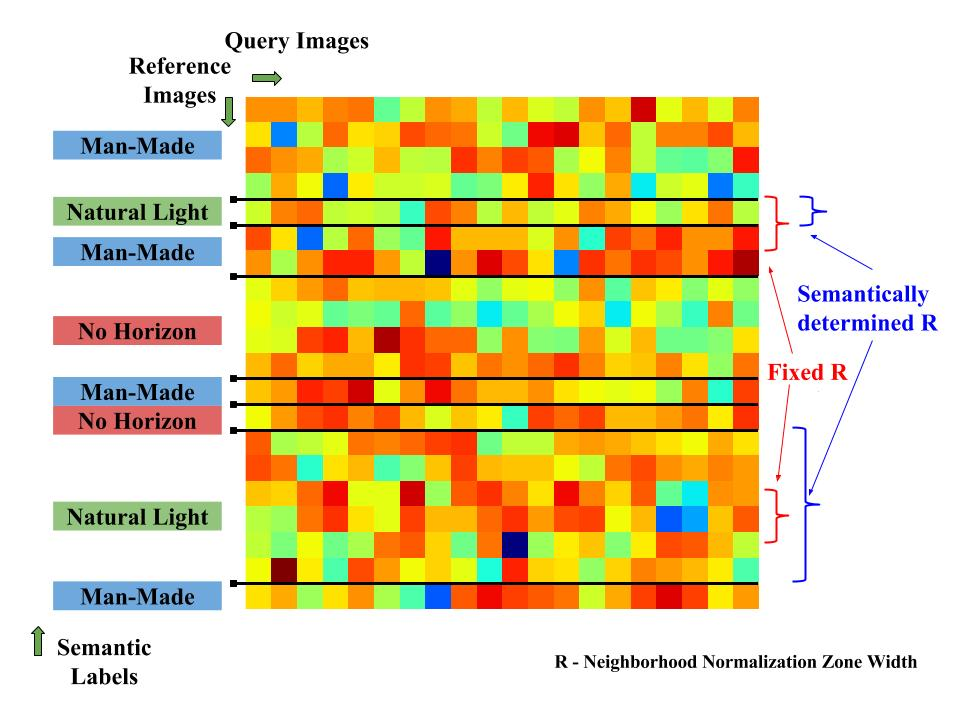
\includegraphics[scale=0.33]{SADmat-NormalisationMethod}
 \caption{The semantic segmentation of environment decides the normalization regions for better place recognition. The matrix represents the Sum of Absolute Difference score between reference and query images of CTA-Rail dataset. The black horizontal lines mark the transitions from one type of environment to the other. The red markers on the right show the fixed neighborhood normalization zone width (R) for SeqSLAM and blue markers refer to the proposed method for determining R.}
 \label{fig:SADmatRdisplay}
\end{figure}

\begin{figure}[h]
\centering
 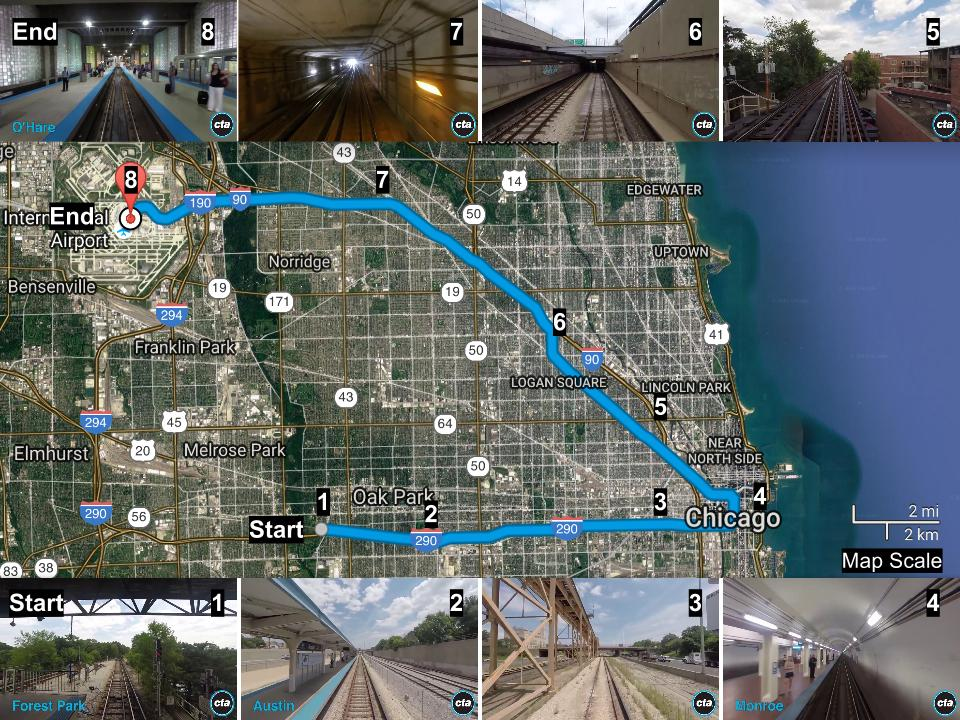
\includegraphics[scale=0.23]{cta-datasetTrajSampleImages}
 \caption{CTA Dataset Trajectory Aerial View with sample images. (Marked Trajectory Source - \cite{ctaTrajGMap})}
 \label{fig:ctaTraj}
\end{figure}

\begin{figure}[h]
\centering
 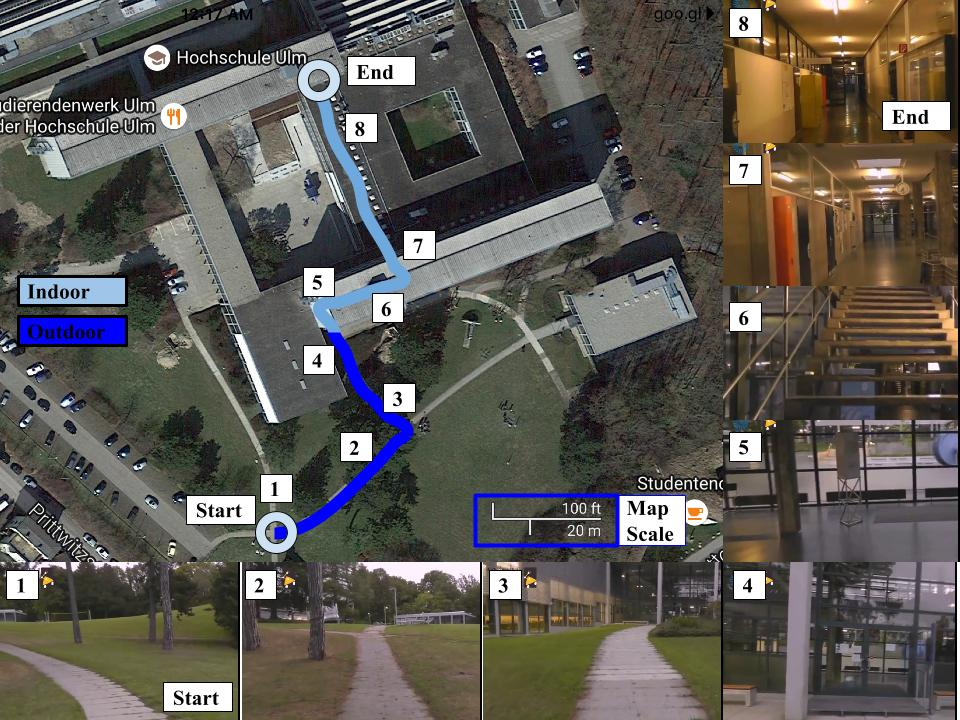
\includegraphics[scale=0.23]{campus-datasetTrajSampleImages}
 \caption{Campus Indoor-Outdoor Dataset Trajectory Aerial View with sample images. (Marked Trajectory Source - \cite{ctaTrajGMap})}
 \label{fig:campusTraj}
\end{figure}

\begin{figure}
\centering
 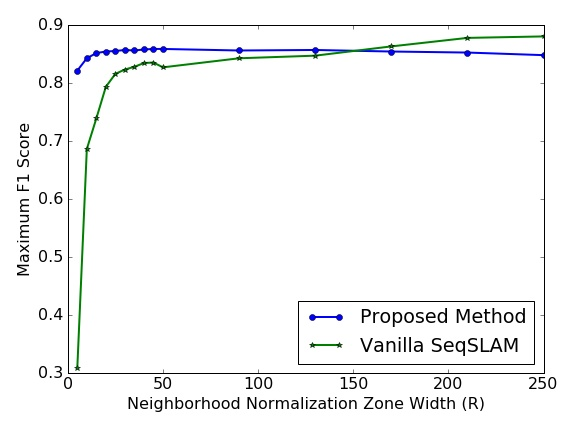
\includegraphics[scale=0.3]{RPerformance1} \\
 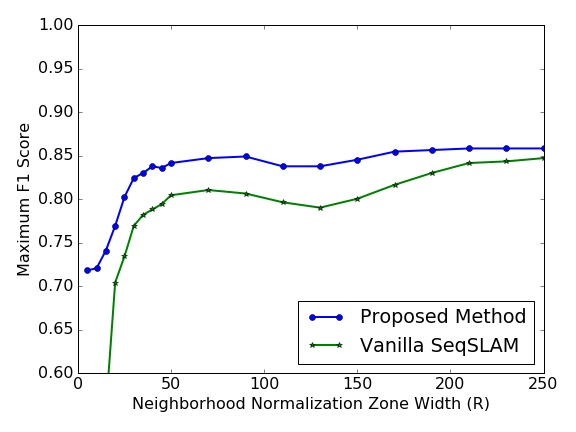
\includegraphics[scale=0.3]{RPerformance2}
 \caption{Performance comparison of proposed method and vanilla SeqSLAM with respect to parameter $R$ for CTA (top) and Campus (bottom) datasets.}
 \label{fig:RPerformance}
\end{figure}


\section{Experimental Setup}
The experiments are performed using two datasets described in a subsequent section. The image classification is performed using a Dell M4800 Intel Core i7, 3.1 GHz processor with NVIDIA Quadro K2100M graphics card. The place recognition is performed using Dell E7450 Intel Core i7, 2.6 GHz processor. The image classification part is done as an off-line preprocessing step for reference and query databases.

\subsection{Datasets}
The two datasets used in the experiments exhibit variations in environmental conditions as the route is traversed.

\subsubsection{CTA-Rail}
The CTA-Rail (Chicago Transit Authority) dataset (Fig. \ref{fig:ctaTraj}) comprises of two videos traversing a 23 km railway route (Blue Line, Forest Park to O'Hare), recorded once in 2014 \cite{ctaRail2014} and then in 2015 \cite{ctaRail2015}, available online. A single camera is placed at the head of the train facing forward toward the railway track. The videos comprise of scenes from train stations platforms, subway station platforms, subway tunnels, and railroad tracks within highways and urban areas. The raw videos are approximately 73 and 84 minutes in duration with 132670 and 149090 frames respectively. We used the 480p version of the video and processed every 200th frame for all the experiments. The resultant reference and query databases have therefore 656 and 738 image frames respectively.

\subsubsection{Campus Indoor-Outdoor}
The Campus Indoor-Outdoor dataset comprises of two videos with repeated traversal of a part of Ulm University of Applied Sciences' campus from an outside lawn to an inside corridor \cite{indoorOutdoor1,indoorOutdoor2}. The videos have been recorded using a hand-held device with single camera and exhibits jerky motion with huge motion blur. The raw videos are cropped to remove the comments at the bottom and an overlaid navigation display on the right side. The videos are also snipped from beginning so that the starting point is aligned in both the datasets. The datasets comprise of scenes from outside the campus, with trees, grass and pavement, and from inside the campus, traversing through entrance hall, staircase, lobby and corridor. The reference and query database is processed by using every 10th image and therefore uses 355 and 300 frames respectively.

\subsubsection{Ground Truth}
The place recognition ground truth for both the datasets was generated manually for intermittent frames and then interpolated for the rest of the image sequence. A query image is considered to be a true positive match for the reference image if its index lies within a range of 5 image frames from the ground truth index.

\subsubsection{SeqSLAM parameters}
The parameters for SeqSLAM used for all the experiments are shown in Table \ref{table:seqSLAMParams}.

\begin{table}[!h]
	\caption{SeqSLAM parameters.}
	\begin{tabular}{|c|p{4cm}|p{2.5cm}|}
		\hline
		$S_x\mathbf{x}S_y$ & Image Down-sampling Size & 32x32 \\
		\hline
		$P$ & Patch Normalization Window Size & {2,4,8,16} \\
		\hline
		$O$ & Image Matching Offset Range & $\pm10$ \\
		\hline
		$d_s$ & Sequence Length & 15 \\
		\hline
		$R$ & Neighborhood Normalization Zone Width & {10,20,40,80,160} \\
		\hline
		$V$ & Sequence Search Velocity Range & $(1\pm0.2)d_s$ \\
		\hline
		$\mu$ & Trajectory Uniqueness Threshold & Varied \\
		\hline
	\end{tabular}
	\label{table:seqSLAMParams}
\end{table}

\section{Results}
We used maximum F1 score to measure changes in place recognition performance using the proposed approach. The trajectory uniqueness parameter (described in \cite{Milford2012}), that is, the threshold for deciding a correctly matched place was varied to calculate precision-recall curve and maximum F1 score. The comparative results were generated between the proposed method and vanilla SeqSLAM for two real world datasets. In order to gain an in-depth understanding of the place recognition performance changes due to proposed approach, we used two parameters of SeqSLAM method, patch normalization window size ($P$) and neighborhood normalization zone width ($R$), to measure the trends in performance change. The results are as shown in Fig. \ref{fig:RPerformance} and \ref{fig:performanceChart}, and the significance and effect of these parameters is discussed in subsequent section. 

Fig. \ref{fig:placeMatches} shows example images that match at the transition point within an environment. It shows the transition for CTA-Rail dataset from inside the tunnel to outside, and for the Campus Indoor-Outdoor dataset from outdoor environment to the indoor. The changes in appearance of environment are evident from the change in lighting and enclosedness.

\newcommand{\imgH}{2.6cm}
\newcommand{\imgW}{4cm}
\begin{figure*}
\centering
 \begin{tabular*}{\textwidth}[t]{cccc}
  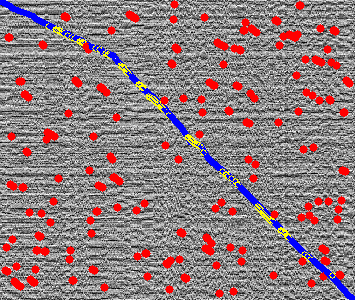
\includegraphics[width=\imgW,height=\imgH]{campus-io-without-bad-101} &
  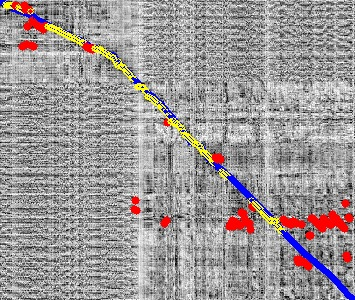
\includegraphics[width=\imgW,height=\imgH]{campus-io-with-bad-71} &
  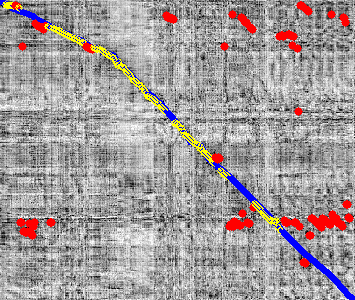
\includegraphics[width=\imgW,height=\imgH]{campus-io-without-good-105} &
  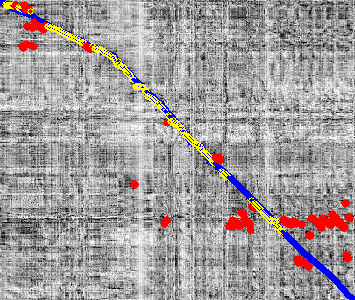
\includegraphics[width=\imgW,height=\imgH]{campus-io-with-good-75} \\
  (a) F Score = 0.46 & (b) F Score = \textbf{0.74} & (c) F Score = 0.72 & (d) F Score = \textbf{0.75} \\
  SeqSLAM & Proposed Approach & SeqSLAM & Proposed Approach \\
  \multicolumn{2}{c}{\textbf{R = 10}, P = 8} & \multicolumn{2}{c}{\textbf{R = 160}, P = 8} \\
  \multicolumn{4}{c}{\emph{Campus Indoor-Outdoor Dataset}} \\
  \\
  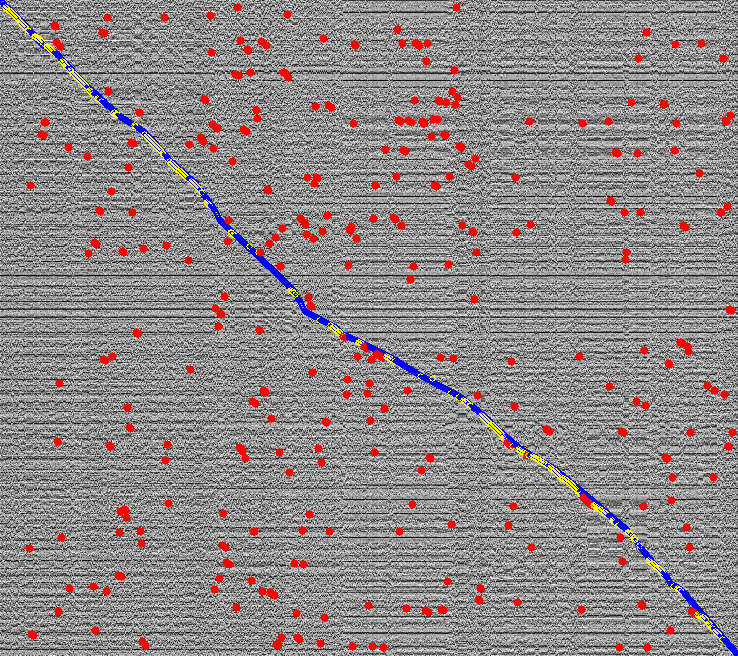
\includegraphics[width=\imgW,height=\imgH]{cta-rail-without-bad-106} &
  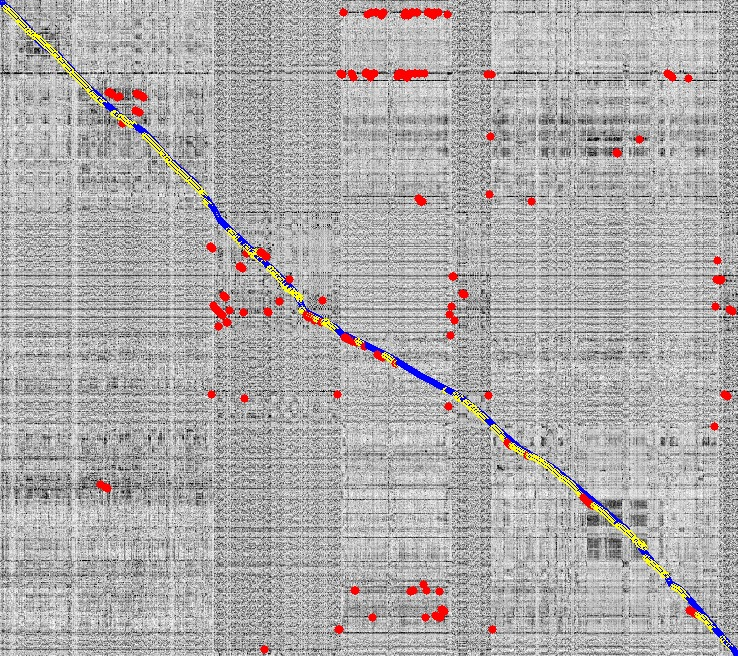
\includegraphics[width=\imgW,height=\imgH]{cta-rail-with-bad-306} &
  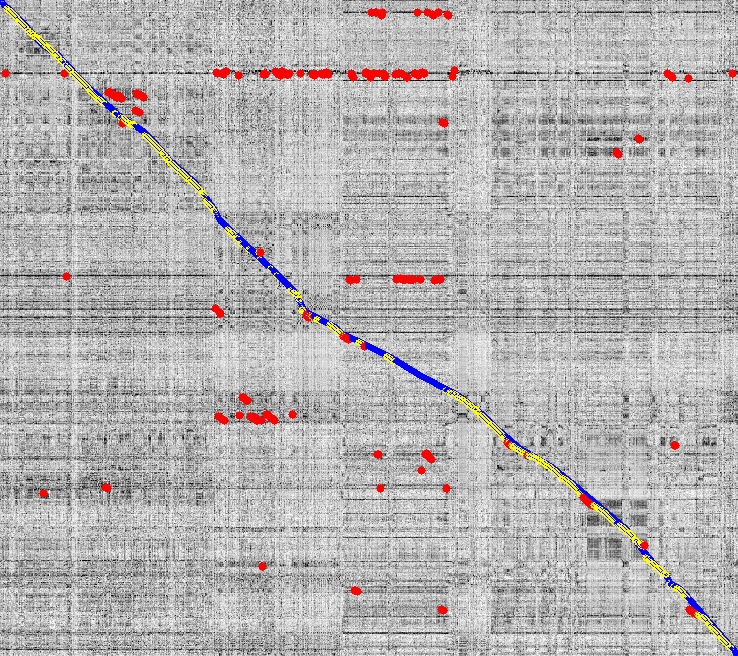
\includegraphics[width=\imgW,height=\imgH]{cta-rail-without-good-110} &
  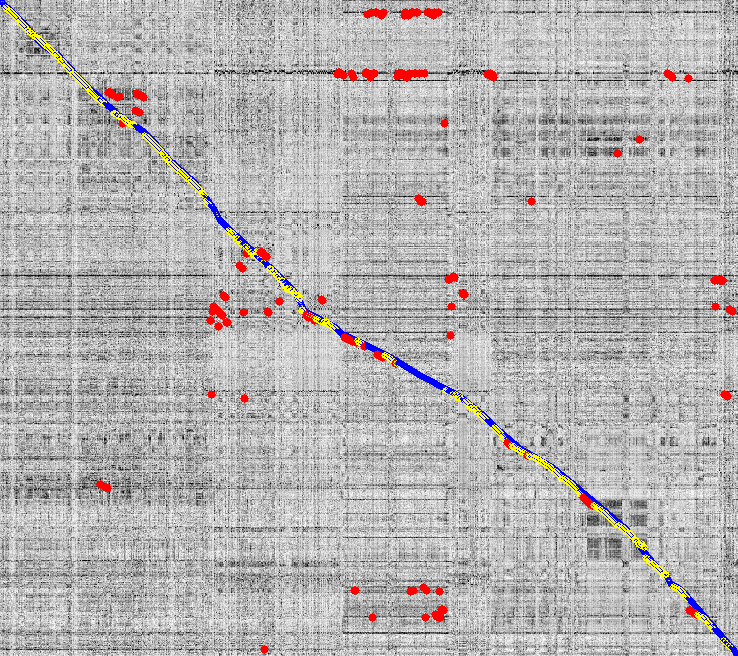
\includegraphics[width=\imgW,height=\imgH]{cta-rail-with-good-310} \\
  (e) F Score = 0.61 & (f) F Score = \textbf{0.82} & (g) F Score = 0.80 & (h) F Score = \textbf{0.82} \\
  SeqSLAM & Proposed Approach & SeqSLAM & Proposed Approach \\
  \multicolumn{2}{c}{\textbf{R = 10}, P = 4} & \multicolumn{2}{c}{\textbf{R = 160}, P = 4} \\
  \multicolumn{4}{c}{\emph{CTA Rail Dataset}}
 \end{tabular*}
 \caption{The SAD (Sum of absolute difference) matrix with reference database as rows and query database as columns. The ground truth is marked in blue, loop closures in red and true positives in yellow. The first and second row corresponds to Campus Indoor-Outdoor and CTA-Rail dataset respectively. Results in (a)-(b) and (e)-(f) correspond to smaller normalization window for vanilla SeqSLAM and proposed approach respectively while (c)-(d) and (g)-(h) correspond to larger normalization window. The dataset segmentation can be seen as rectangular dark and light patches. The images here show that performance improvement is significant for smaller values of R, whereas, with larger R values, performance of vanilla SeqSLAM method approaches to that of proposed method.}
 \label{fig:sadMat}

\end{figure*}


\begin{figure}
\centering
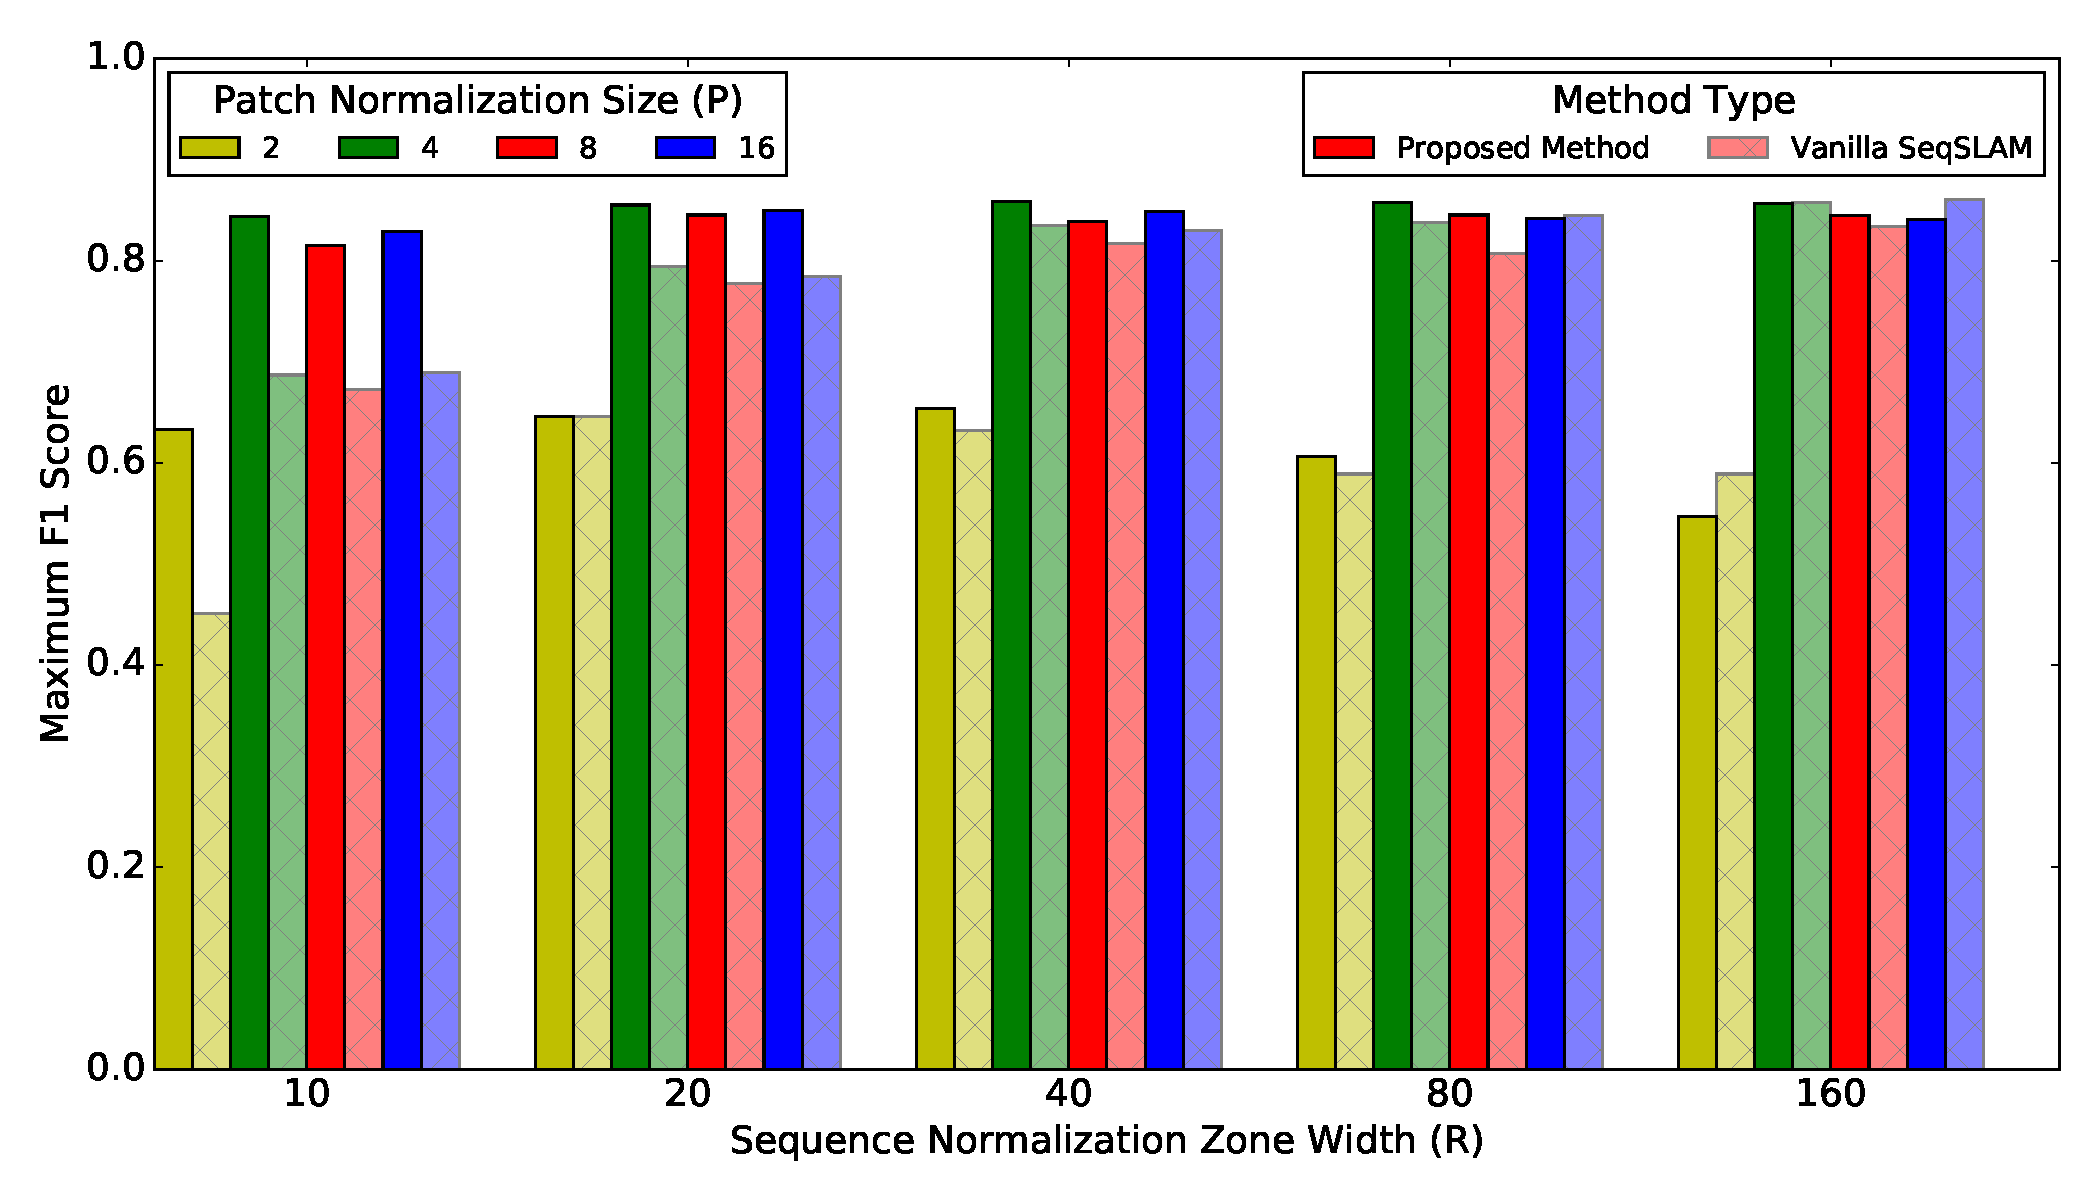
\includegraphics[scale=0.48]{cta-bar-graph}\\
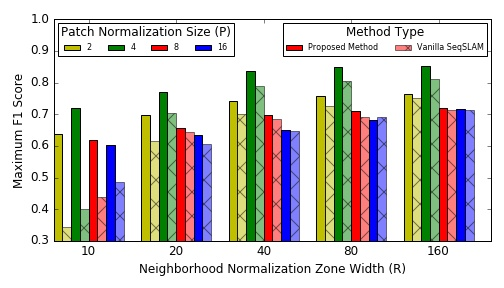
\includegraphics[scale=0.48]{campus-io-bar-graph}
 \caption{Performance chart showing maximum F1 Score. The first row corresponds to the CTA-Rail dataset and second row to the Campus Indoor-Outdoor dataset. The performance improves with increasing the parameter value R, where vanilla SeqSLAM performs equally good as the proposed approach. The patch normalization window size ($P$) parameter with value 4 happens to perform better as compared to others.}
 \label{fig:performanceChart}
\end{figure}

Figure \ref{fig:sadMat} shows the ground truth and the place recognition matches (without thresholding) corresponding to different parameter settings for both vanilla SeqSLAM and proposed method. The performance improvement is large for both the datasets for smaller values of $R$ (neighborhood normalization zone width). The large $R$ values help the vanilla method to attain performance equivalent to the proposed approach as shown in Figure \ref{fig:sadMat}. The effect of dataset segmentation can be easily seen and understood in the these images in form of rectangular dark and light patches in the SAD matrix. 


\section{Discussion and Future Work}
In this work, we presented a framework which combines place categorization information to inform and improve place recognition results. The system was tested by using two real world datasets, highlighting the proposed system's superiority over a state-of-the-art place recognition system. Here, we discuss the effects of system parameters, the improvements achieved by the proposed approach and potential extensions and future work for this approach. 

\subsection{Effect of SeqSLAM parameters}
\subsubsection{Neighborhood Normalization Zone Width ($R$)}
The neighborhood normalization parameter $R$ is used to set the window size for locally enhancing the match scores. As shown in Figure \ref{fig:performanceChart}, performance of vanilla SeqSLAM gets better with an increase in $R$. This can be expected because normalizing over a larger image sequence balances the overall variation in scores for varying conditions within an environment, but it leads to suppressing of correct matching pairs corresponding to images having low matching scores, especially in the smaller zones. On the other hand, using segmented regions to set the normalization zone width, effectively highlights the matching scores in appropriate regions and generates more true positives. The performance is, therefore, most of the times, better than the best achieved using vanilla approach with any value of $R$. It can also be noted that wider neighborhood zones for normalization, are not appropriate for large datasets and long time navigation due to computational burden. 

\subsubsection{Patch Normalization Window Size ($P$)}
The images used for finding SAD score are preprocessed by down-sampling them to the size of $32\mathbf{x}32$ and then patch normalized in order to counter the changes in appearance of their matching counterparts. Depending on the type of environment and corresponding imagery, the choice of patch normalization window size can lead to changes in performance. In the experiments performed for current work, we found that patch normalization window size of 4 for the given down-sampling image size performs better.

\subsection{Physical Space Segmentation}
Fig. \ref{fig:RPerformance} shows a performance comparison for both the datasets with respect to the parameter $R$ alone. The curves here give us an insight to understand how an optimal value for segmenting the physical space can be chosen. For both the datasets, the performance of vanilla SeqSLAM and the proposed approach becomes almost similar at a certain point, beyond which no significant improvement occurs. This happens when $R$ is approximately between 20 and 25, which is almost 1 km of journey in the CTA Rail dataset captured at speed of train and about 50 m for Campus dataset captured at normal human speed. The visual data captured in both the cases is therefore sufficient enough to correctly segment its physical space. If the physical region spanned were to be smaller than this, it would have created an inter-region redundancy of visual data which would mean more confusing matching places. Hence, the optimal value for segmenting the environment would be based on the average rate of persistence of particular environmental conditions. However, it would still fail for the cases where there is a large variance in the span of different conditions existing within the environment, and a proper segmented environment based on semantic information will be the key to perform better.

\subsection{Environmental Transitions}
We have demonstrated performance improvement for a place recognition system by appropriately handling different visual conditions within an environment, but one also needs to be careful about the exact point of transition within these different conditional settings. In general, there is a sequence of images, that are encountered, for example, while moving from outside the tunnel to inside the tunnel and vice versa. The current state-of-the-art place categorization module trained on limited number of places or scene attributes cannot always effectively discriminate the exact transition point/region from the environments between which the transition takes place. This leads to false matching of possibly false semantic labels and hence poor performance at those points. Moreover, in our current approach, the transition areas, that span only few images, also get ignored during the label filtering process. Though, it can be taken care of by using smaller filtering window size $s$ (described in earlier sections), but then it would demand correct semantic labels with temporal consistency. This problem makes more sense to be solved from the place categorization side, by training place categories at a further fine level, such that being inside the tunnel or outside of it is also discriminated from starting to seeing the tunnel entry or the exit, which actually marks the transition to a new environment, and thus becomes a part of our future work.


\subsection{Future Work}
The current work can be extended to incorporate labels of place categories or scene attributes defined at finer levels, as also discussed in previous section. Such fine level place categorization will be directed towards the traditional place recognition problem where each place, despite being from same semantic category, is treated as a separate place. It would also be worth exploring ways to dynamically determine the sequence length for matching places while using the semantic place information.  We would also like to investigate better ways of generating semantic labels with temporal coherence, given that the research problems of object recognition and place categorization usually focus on single images instead of image sequences. Another interesting direction could be a deep-learning framework, using a combination of LSTM and CNN to effectively exploit the temporal and spatial information respectively and infer relationship between places with similar visual appearances.



%\section{Conclusion}

%\addtolength{\textheight}{-8cm}   % This command serves to balance the column lengths
                                  % on the last page of the document manually. It shortens
                                  % the textheight of the last page by a suitable amount.
                                  % This command does not take effect until the next page
                                  % so it should come on the page before the last. Make
                                  % sure that you do not shorten the textheight too much.

%\section*{ACKNOWLEDGMENT}

%The preferred spelling of the word ÒacknowledgmentÓ in America is without an ÒeÓ after the ÒgÓ. Avoid the stilted expression, ÒOne of us (R. B. G.) thanks . . .Ó  Instead, try ÒR. B. G. thanksÓ. Put sponsor acknowledgments in the unnumbered footnote on the first page.

\bibliographystyle{IEEEtran}
\bibliography{IEEEabrv,ral-icra-2017}

\end{document}
